\chapter{Algorithmic Model}
\label{sec:architectureAndModel}
The suggested algorithm is a new hybrid approach for combining the island model with AIS. The proposed approach to this, is to initialise each island with its own AIS. The combined algorithm will take parameters for both of the techniques, as explained in the sections below. Additionally, some parameters like termination condition, will be given to the algorithm as a whole.

\section{IGA Configuration}

%guess you defined IGA as Island GA somewhere? 

The current state of the art of combining IGA and AIS is very vague or not existing, therefor the most rational approach will be to keep the configuration of IGA very general. This implies following the most common ways of structuring the model.

\subsection{Structure - Topology}
%should be called a directed ring topology, given that there is only one direction. Maybe this terminology hasn't been used in AIS?
%island doesn't migrate...it is individuals.. 
The islands will be structured following a ring topology, where each island can only migrate to one specific island, as well as receive immigrants from one specific island (see figure \ref{fig:iga:ring-model}). The number of islands will be passed in as a parameter to the algorithm during its initialisation, however the ring topology will always yield. As discussed in section \ref{sec:motivation:iga}, this topology has proved good results in terms of rapid convergence, as well as preventing premature convergence. This topology is also recognised as simple, which is a good initial condition when trying to combine it with other techniques.    


\begin{figure}
    \centering
    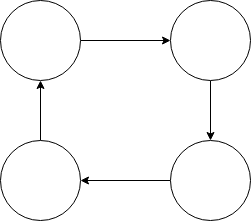
\includegraphics[width=0.3\columnwidth]{figs/ring-model.png}
    \caption{Basic island model with ring topology}
    \label{fig:iga:ring-model}
\end{figure}

% i geuss this figure is given earlier and since it doesn't give any new information then you can just refer back to the earlier version. Makes more sense to introduce it earlier, especailly since it is not your direct contribution. Have you stated somewhere with citations that the ring is the most common form? If not do so. 
%Guess you also have described the concept of simple somewhere earlier with cites. What gives this topology its simplicity. 4 rings fully connected could be said to be simple too. 


\subsection{Migration Policy}

%cover essential standards.....not sure what this means.... follow the normal...btu strange expression. Cut the first sentence, deosn't say anything. 
\subsection{IGA Parameters}
The parameters defined for the IGA will cover essential standards for the current technique. This will include number of islands, which individuals to migrate and when to migrate them. 

%need to be careful som to which parameters are part of the IGA and what are part of the AIS. The iGA does have individuals ie chromosones, operators and populations etc. Especially population on each island must be an island parameter. 

\section{AIS Configuration}

\subsection{Chromosome Structure}

% simplify these explanations. What are the model features - say them clearly. What are the justifications - state these clearly but make sure that these different elements are seperated so you can't clearly pick out the elements of the model. Also there is a mixture of justifications in the previous chapter and here. Need to find a clear process here as to where the justifications should be. just a bit mixed up at the moment. 
%Basically you are introducing a variable length chromosone to account for different subsets of features plus a gene representing the radius of the chromosone. 
%diagram please of the chromosone
%explanation of how the local feature selection will happen - somewhere. 
%surely you also have a chromosone structure for an Antigen even though your population is made of Antibodies. 
Since some of the data sets used for experiments will have quite high feature count per case it is likely that the curse of dimensionality will cause problems for the algorithm as discussed in section \ref{sec:motivation_ais}. Therefore the algorithm will employ local feature selection to address this (also mentioned in \ref{sec:motivation_ais}). This means that the different antibody chromosomes will not have the same structure as e.g. one antibody may consist of two features of the total feature space of thirty, while another antibody employ ten of those features. Additionally, a hypersphere will be used for the shape of the recognition zone so each chromosome will also include a radius. 

\subsection{Crossover}
% Are you then using cloning, mutation and crossover. If so state it. 
While most AIS algorithms employ a scheme of cloning and mutation this algorithm will apply a crossover to the antibodies. This is because the algorithm uses an island model structure, and with this structure antibodies will be moved between the islands. If you apply only cloning on this model the islands will have no effects as no matter which island you perform clone the antibody on the result will always be the same as cloning does not interact with other antibodies on the island. However, how migrating individuals change the population on the islands they arrive on is vital to an IGA, so some form of interaction is necessary. Therefore, crossover is chosen for this purpose. 

\subsection{Fitness Calculation}

\subsection{Mutation}


\subsection{AIS Parameters}
The parameters will be standard parameters of most evolutionary algorithm like, crossover and mutation rate, population size and number of iterations, as well as initial conditions for the antibodies such as numerical ranges of feature count and radius. 

%you are already discussing AIS parameters above so a subsection called AIS parameters seems redundant. 
%Although you are far from finished writing this section make sure you really introduce the model.You might want to keep all your discussions to the previous chapters and here just state the features of the model clearly.  

\section{Termination}
The algorithm terminates when the it reaches the maximum number of iterations, the algorithm prematurely converges and considerable efforts to stop this does not sufficiently do so or when the algorithm achieves a sufficiently optimal solution.


